\documentclass[a4paper,11pt]{book}
%\documentclass[a4paper,twoside,11pt,titlepage]{book}
\usepackage{listings}
\usepackage[utf8]{inputenc}
\usepackage[spanish]{babel}

% \usepackage[style=list, number=none]{glossary} %
%\usepackage{titlesec}
%\usepackage{pailatino}

\decimalpoint
\usepackage{dcolumn}
\newcolumntype{.}{D{.}{\esperiod}{-1}}
\makeatletter
\addto\shorthandsspanish{\let\esperiod\es@period@code}
\makeatother


%\usepackage[chapter]{algorithm}
\RequirePackage{verbatim}
%\RequirePackage[Glenn]{fncychap}
\usepackage{fancyhdr}
\usepackage{graphicx}
\usepackage{afterpage}

\usepackage{longtable}

\usepackage[pdfborder={000}]{hyperref} %referencia

% ********************************************************************
% Re-usable information
% ********************************************************************
\newcommand{\myTitle}{Título del proyecto\xspace}
\newcommand{\myDegree}{Grado en ...\xspace}
\newcommand{\myName}{Nombre Apllido1 Apellido2 (alumno)\xspace}
\newcommand{\myProf}{Nombre Apllido1 Apellido2 (tutor1)\xspace}
\newcommand{\myOtherProf}{Nombre Apllido1 Apellido2 (tutor2)\xspace}
%\newcommand{\mySupervisor}{Put name here\xspace}
\newcommand{\myFaculty}{Escuela Técnica Superior de Ingenierías Informática y de
Telecomunicación\xspace}
\newcommand{\myFacultyShort}{E.T.S. de Ingenierías Informática y de
Telecomunicación\xspace}
\newcommand{\myDepartment}{Departamento de ...\xspace}
\newcommand{\myUni}{\protect{Universidad de Granada}\xspace}
\newcommand{\myLocation}{Granada\xspace}
\newcommand{\myTime}{\today\xspace}
\newcommand{\myVersion}{Version 0.1\xspace}


\hypersetup{
pdfauthor = {\myName (email (en) ugr (punto) es)},
pdftitle = {\myTitle},
pdfsubject = {},
pdfkeywords = {palabra_clave1, palabra_clave2, palabra_clave3, ...},
pdfcreator = {LaTeX con el paquete ....},
pdfproducer = {pdflatex}
}

%\hyphenation{}


%\usepackage{doxygen/doxygen}
%\usepackage{pdfpages}
\usepackage{url}
\usepackage{colortbl,longtable}
\usepackage[stable]{footmisc}
%\usepackage{index}

%\makeindex
%\usepackage[style=long, cols=2,border=plain,toc=true,number=none]{glossary}
% \makeglossary

% Definición de comandos que me son tiles:
%\renewcommand{\indexname}{Índice alfabético}
%\renewcommand{\glossaryname}{Glosario}

\pagestyle{fancy}
\fancyhf{}
\fancyhead[LO]{\leftmark}
\fancyhead[RE]{\rightmark}
\fancyhead[RO,LE]{\textbf{\thepage}}
\renewcommand{\chaptermark}[1]{\markboth{\textbf{#1}}{}}
\renewcommand{\sectionmark}[1]{\markright{\textbf{\thesection. #1}}}

\setlength{\headheight}{1.5\headheight}

\newcommand{\HRule}{\rule{\linewidth}{0.5mm}}
%Definimos los tipos teorema, ejemplo y definición podremos usar estos tipos
%simplemente poniendo \begin{teorema} \end{teorema} ...
\newtheorem{teorema}{Teorema}[chapter]
\newtheorem{ejemplo}{Ejemplo}[chapter]
\newtheorem{definicion}{Definición}[chapter]

\definecolor{gray97}{gray}{.97}
\definecolor{gray75}{gray}{.75}
\definecolor{gray45}{gray}{.45}
\definecolor{gray30}{gray}{.94}

\lstset{ frame=Ltb,
     framerule=0.5pt,
     aboveskip=0.5cm,
     framextopmargin=3pt,
     framexbottommargin=3pt,
     framexleftmargin=0.1cm,
     framesep=0pt,
     rulesep=.4pt,
     backgroundcolor=\color{gray97},
     rulesepcolor=\color{black},
     %
     stringstyle=\ttfamily,
     showstringspaces = false,
     basicstyle=\scriptsize\ttfamily,
     commentstyle=\color{gray45},
     keywordstyle=\bfseries,
     %
     numbers=left,
     numbersep=6pt,
     numberstyle=\tiny,
     numberfirstline = false,
     breaklines=true,
   }
 
% minimizar fragmentado de listados
\lstnewenvironment{listing}[1][]
   {\lstset{#1}\pagebreak[0]}{\pagebreak[0]}

\lstdefinestyle{CodigoC}
   {
	basicstyle=\scriptsize,
	frame=single,
	language=C,
	numbers=left
   }
\lstdefinestyle{CodigoC++}
   {
	basicstyle=\small,
	frame=single,
	backgroundcolor=\color{gray30},
	language=C++,
	numbers=left
   }

 
\lstdefinestyle{Consola}
   {basicstyle=\scriptsize\bf\ttfamily,
    backgroundcolor=\color{gray30},
    frame=single,
    numbers=none
   }


\newcommand{\bigrule}{\titlerule[0.5mm]}


%Para conseguir que en las páginas en blanco no ponga cabecerass
\makeatletter
\def\clearpage{%
  \ifvmode
    \ifnum \@dbltopnum =\m@ne
      \ifdim \pagetotal <\topskip
        \hbox{}
      \fi
    \fi
  \fi
  \newpage
  \thispagestyle{empty}
  \write\m@ne{}
  \vbox{}
  \penalty -\@Mi
}
\makeatother

\usepackage{pdfpages}
\begin{document}
\begin{titlepage}
 
 
\newlength{\centeroffset}
\setlength{\centeroffset}{-0.5\oddsidemargin}
\addtolength{\centeroffset}{0.5\evensidemargin}
\thispagestyle{empty}

\noindent\hspace*{\centeroffset}\begin{minipage}{\textwidth}

\centering

\includegraphics[width=0.9\textwidth]{imagenes/logo_ugr.eps}\\[1.4cm]


\textsc{ \Large TRABAJO FIN DE GRADO\\[0.2cm]}
\textsc{INGENIERÍA DE TECNOLOGÍAS DE TELECOMUNICACIÓN}\\[1cm]
% Upper part of the page
% 
% Title
{\Huge\bfseries  Sistema de
	control autónomo para robots en FPGAs de
	software libre\\
}
\noindent\rule[-1ex]{\textwidth}{3pt}\\[3.5ex]
{\large\bfseries } %Aqui el subtitulo
\end{minipage}

\vspace{1cm}
\noindent\hspace*{\centeroffset}\begin{minipage}{\textwidth}
\centering

\textbf{Autor}\\ {Juan Ordóñez Cerezo}\\[2.5ex]
\textbf{Directores}\\
{Encarnación del Castillo Morales\\
Jose María Cañas Plaza}\\[2cm]

\includegraphics[width=0.3\textwidth]{imagenes/etsiit_logo.png}\\[0.1cm]
\textsc{Escuela Técnica Superior de Ingenierías Informática y de Telecomunicación}\\
\textsc{---}\\
Granada, Noviembre de 2018
\end{minipage}
%\addtolength{\textwidth}{\centeroffset}
%\vspace{\stretch{2}}
\end{titlepage}



\chapter*{}
%\thispagestyle{empty}
%\cleardoublepage

%\thispagestyle{empty}

\begin{titlepage}
 
 
\setlength{\centeroffset}{-0.5\oddsidemargin}
\addtolength{\centeroffset}{0.5\evensidemargin}
\thispagestyle{empty}

\noindent\hspace*{\centeroffset}\begin{minipage}{\textwidth}

\centering
%
\includegraphics[width=0.9\textwidth]{imagenes/logo_ugr.jpg}\\[1.4cm]



 \vspace{3.3cm}

%si el proyecto tiene logo poner aquí
%
\includegraphics{imagenes/logo.png} 
 \vspace{0.5cm}

% Title

{\Huge\bfseries  Control system in open FPGAs for autonomous robots.\\
}
\noindent\rule[-1ex]{\textwidth}{3pt}\\[3.5ex]
 %Subtitulo de nuevo
\end{minipage}

\vspace{2.5cm}
\noindent\hspace*{\centeroffset}\begin{minipage}{\textwidth}
\centering

\textbf{Author}\\ {Juan Ordóñez Cerezo}\\[2.5ex]
\textbf{Directors}\\
{Encarnación del Castillo Morales\\
Jose María Cañas Plaza}\\[2cm]
%
\includegraphics[width=0.15\textwidth]{imagenes/tstc.png}\\[0.1cm]
%\textsc{Departamento de Teoría de la Señal, Telemática y Comunicaciones}\\
%\textsc{---}\\
%Granada, mes de 201
\end{minipage}
%\addtolength{\textwidth}{\centeroffset}
\vspace{\stretch{2}}

 
\end{titlepage}






\cleardoublepage
\thispagestyle{empty}

\begin{center}
{\large\bfseries  Control system in open FPGAs for autonomous robots.}\\
\end{center}
\begin{center}
Juan Ordóñez Cerezo\\
\end{center}

%\vspace{0.7cm}
\noindent{\textbf{Key words}: FPGA, IceStudio, IceZumAlhambra, microcontroller, Self-Balancing, quadcopter, OpenSource.}\\

\vspace{0.7cm}
\noindent{\textbf{Abstract}}\\

This paper proposes a new use of FPGAs in educational robotics field. For that, different robotic behaviors are being developed creating a module library that is useful and giving their user the possibility to work at a high abstraction level. As an example, a self-balance robot is proposed and which explanation consists about this project. Without loosing sight of the initial finality, tools used for that will be in the open source community, as can be IceStudio and IceZum Alhambra.
\cleardoublepage

\chapter*{}
\thispagestyle{empty}

\noindent\rule[-1ex]{\textwidth}{2pt}\\[4.5ex]

Me, \textbf{Juan Ordóñez Cerezo}, student of the degree in Telecommunications Technologies Engineering from \textbf{Escuela Técnica Superior
de Ingenierías Informática y de Telecomunicación de la Universidad de Granada}, with DNI 77143207-B, authorize the location of my Final Degree Thesis in the library of the center so that it can be consulted by people who need it.

\vspace{6cm}

\noindent Fdo: Juan Ordóñez Cerezo

\vspace{2cm}

\begin{flushright}
Granada on November 19, 2018.
\end{flushright}


\chapter*{}
\thispagestyle{empty}

\noindent\rule[-1ex]{\textwidth}{2pt}\\[4.5ex]

D. \textbf{Encarnación del Castillo Morales}, Teacher from Electronic Area of the Electronic Department and Computer Technology from Granada University.

\vspace{0.5cm}

D. \textbf{Jose María Cañas Plaza}, Teacher from Theory of Signal and Communications and Telematic Systems and Computing department from Universidad Rey Juan Carlos, Madrid.


\vspace{0.5cm}

\textbf{Inform:}

\vspace{0.5cm}

That the present project, titled \textit{\textbf{Autonomous control system for Robots in FPGA}},
has been developed under supervision by \textbf{Juan Ordóñez Cerezo}, and we authorize the defense from this project in front of the corresponding tribunal.

\vspace{0.5cm}

And for the record, the report has been issued and signed in Granada on November 19, 2018.

\vspace{1cm}

\textbf{The directors:}

\vspace{5cm}

\noindent \textbf{Encarnación del Castillo Morales\ \ \ \ \ Jose María Cañas Plaza}

\chapter*{Acknowledgements}
\thispagestyle{empty}

       \vspace{1cm}

In first place, and for that reason the most important, I want to thank my family, {\bf Juan, Paqui and María}, who have suffered and enjoyed this project as much as I have, for their credibility, patience, for the moments of weakness supplied with joy and above all for believing in the capacity of someone who never gave reasons for it.\newline
Of course, to my tutors Jose María Cañas Plaza and Encarnación del Castillo Morales who believed and made me believe since the beginning in this project and who have taken me to what I am now. \newline
To my colleagues and friends from Munich, from Eesy Innovation and Infineon Technologies, who turned last summer into the best summer in the world and who helped me without asking why, because if something has to go right, it would come out all right.\newline
To my friends from Granada whom I have had to say so many times not because of spending time, but because I never get tired of being with them and because they cheered me up with laughter and jokes.\newline
Finally, I remember part of the speech of two professors in my graduation, two professors, who not just for being teachers forget to treat us as people and who saw us cry, laugh and above all, to grow up. And, if I have to take something from here, it's not only the knowledge learned, it's the friends and those people who help you climb when you do not have the strength to keep climbing, people who believe in you even when you've fallen a few times. \newline
{\bf For all of that, thanks.}

\vspace{1cm}

{\bf Granada on November 19, 2018.}


%\frontmatter
%\tableofcontents
%\listoffigures
%\listoftables
%
%\mainmatter
%\setlength{\parskip}{5pt}

%\chapter{Introducción}\label{sec:intro}
\subsection{Motivación y objetivos}
La electrónica digital forma parte de la rama de electrónica mas moderna y que evoluciona más rápidamente de la actualidad, debido a las ventajas de esta y las cuáles serán analizadas en el presente proyecto. Por ello, es importante llevar a todo el mundo esta tecnología, hacerla amigable y dotar a la sociedad de las herramientas necesarias para su correcto entendimiento, sin que ello suponga la realización de unos estudios superiores. \newline

Involucrarse de lleno en un proyecto tan poco desarrolado y con tan poco información, puede parecer un poco abrumador en principio, sobretodo cuando los problemas empiezan a aparecer, pero para cualquier ingeniero es todo un reto poder empezar a abrir camino sobre un campo determinado, ofreciendo a la sociedad algunas herramientas útiles para futuras implementaciones. \newline

Trabajar sobre una plataforma nativa de tu ciudad como es la IceZum Alhambra teniendo en cuenta el poco desarrollo en este campo, es además un honor que no hay que perder de vista a la hora de definir las motivaciones y objetivos. \newline

Electrónica digital, FPGAs, micro-controlador, lenguaje de descripción hardware, son sólo algunos de los conceptos más importantes sobre los que se sustentan el presente trabajo, y forma parte también de una de las más importantes líneas de investigación sobre ingenieros de todo el mundo. Es un objetivo poder llevar este concepto a las aulas de los más pequeños de la sociedad, haciendo uso para ello de librerías de bloques de implementación hardware que ayudarán en los sucesivos trabajos y abriendo el concepto de "robótica educativa". \newline

A continuación se presentan los objetivos más importantes del presente trabajo:
\begin{itemize}
	
\end{itemize}

\subsection{Planificación (Diagrama de Gantt)}

\begin{center}
	\begin{figure}[H]
		\center
		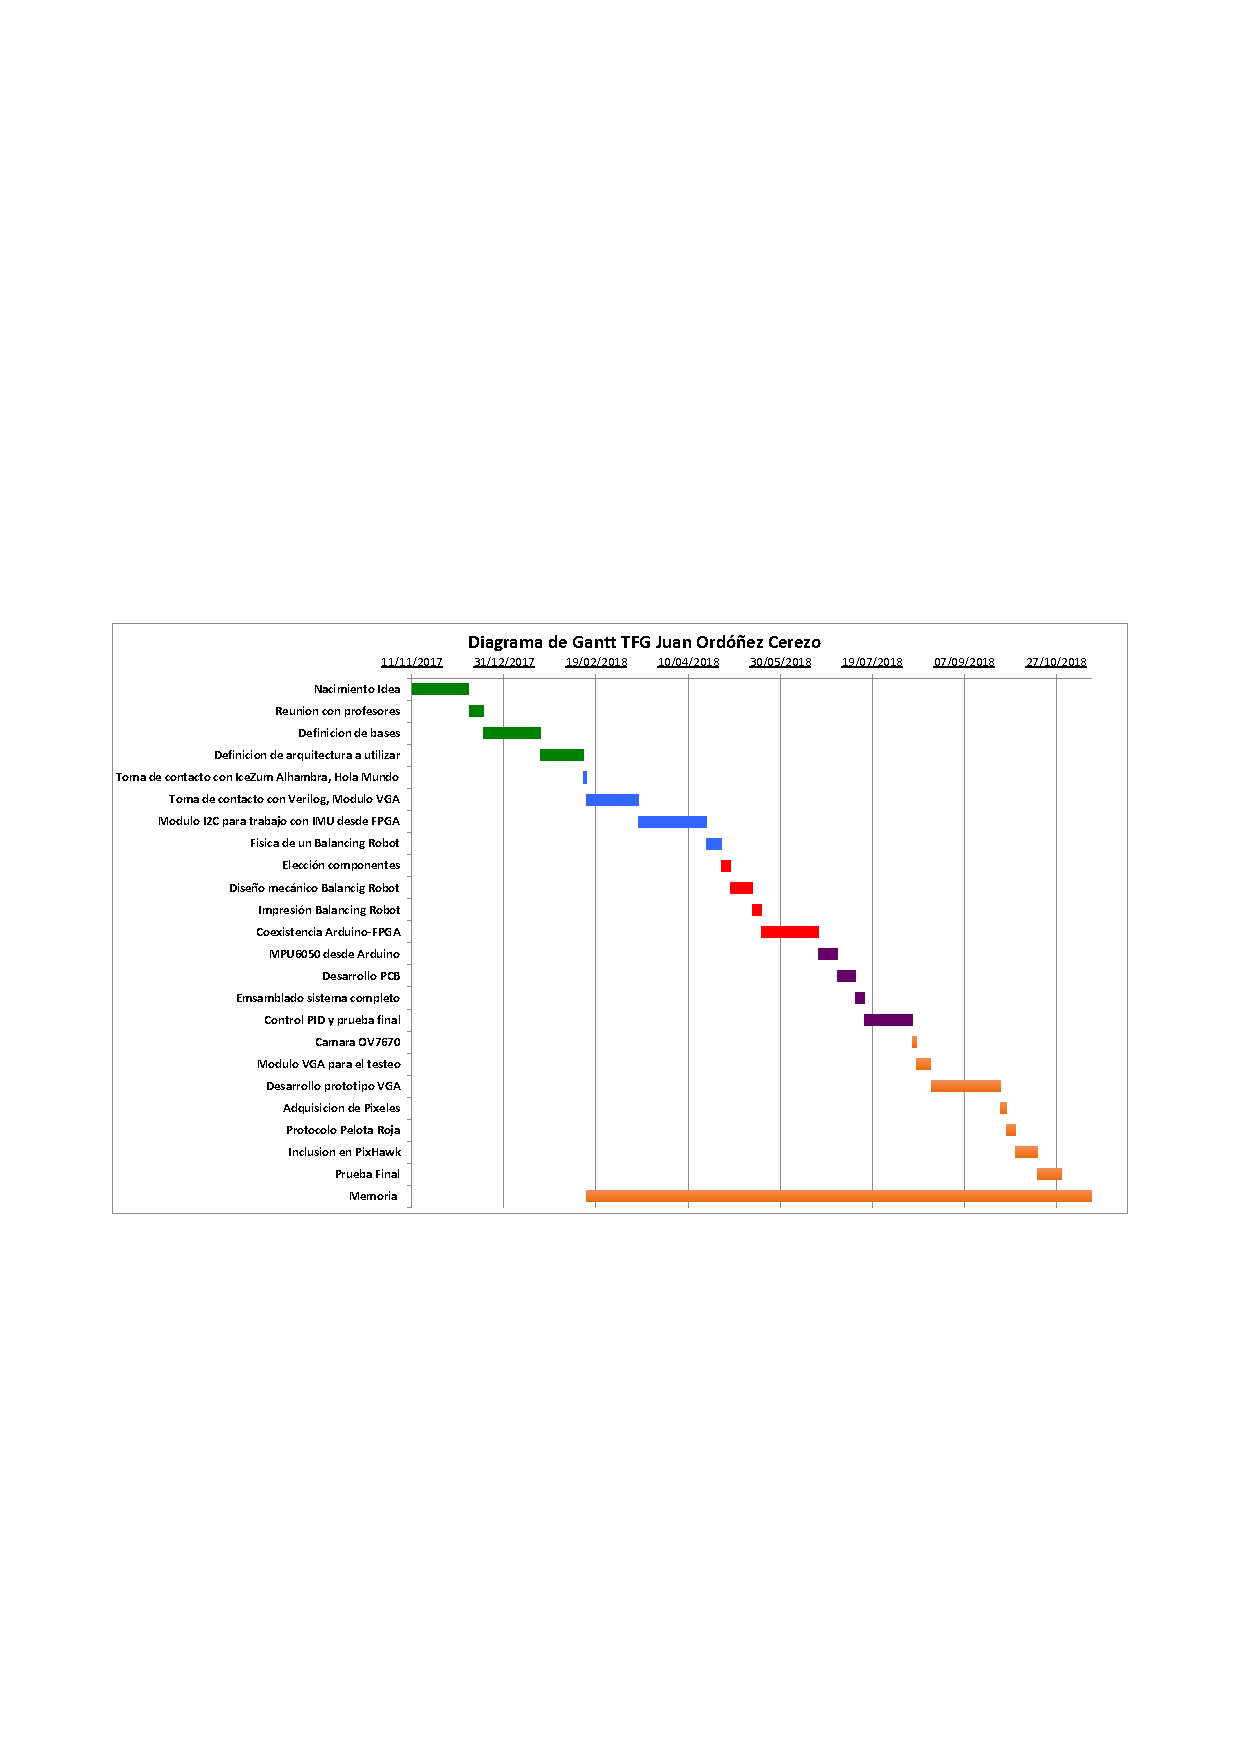
\includegraphics[trim = 15mm 85mm 0mm 100mm,clip, angle=-90, scale = 1.4]{imagenes/Introduction/Gantt.pdf}
		\label{fig:diagramaGantt}
	\end{figure}
\end{center}
\subsection{Metodología de trabajo}
Para introducir la metodología de trabajo seguida, se presenta la herramienta GitHub (figura \ref{fig:github}).\newline 

\begin{figure}[H]
	\center
	
\includegraphics[trim = 0mm 0mm 0mm 0mm, clip,scale=0.4]{imagenes/Introduction/github}
	\caption{Logo GitHub.}
	\label{fig:github}
\end{figure}


GitHub es una plataforma de desarrollo colaborativo de software para alojar proyectos utilizando el sistema de control de versiones Git. GitHub aloja tu proyecto en un repositorio y brinda herramientas muy útiles para el trabajo en equipo. \newline
Proporciona además la posibilidad de una Wiki para el mantenimiento de las versiones e información acerca de ellas. \newline
En el presente proyecto GitHub ha sido usado como un contenedor, donde se ha ido subiendo todo de manera parcial, normalmente, cuando se obtenía una versión estable sobre algunas de las ramas. \newline
De esta forma, y al ser abierto, cualquier persona ha podido seguir los avances de este, dudas, problemas, o incluso utilizar algunos de los módulos o material subidos. \newline
 
El proyecto puede encontrarse en la siguiente URL: \newline

\hyperref[]{https://github.com/RoboticsURJC-students/2017-tfg-juan-ordonez}

Un ejemplo de la trayectoria de este proyecto se representa en la captura de pantalla de GitHub en la figura \ref{fig:capturaGit}.

\begin{figure}[H]
	\center
	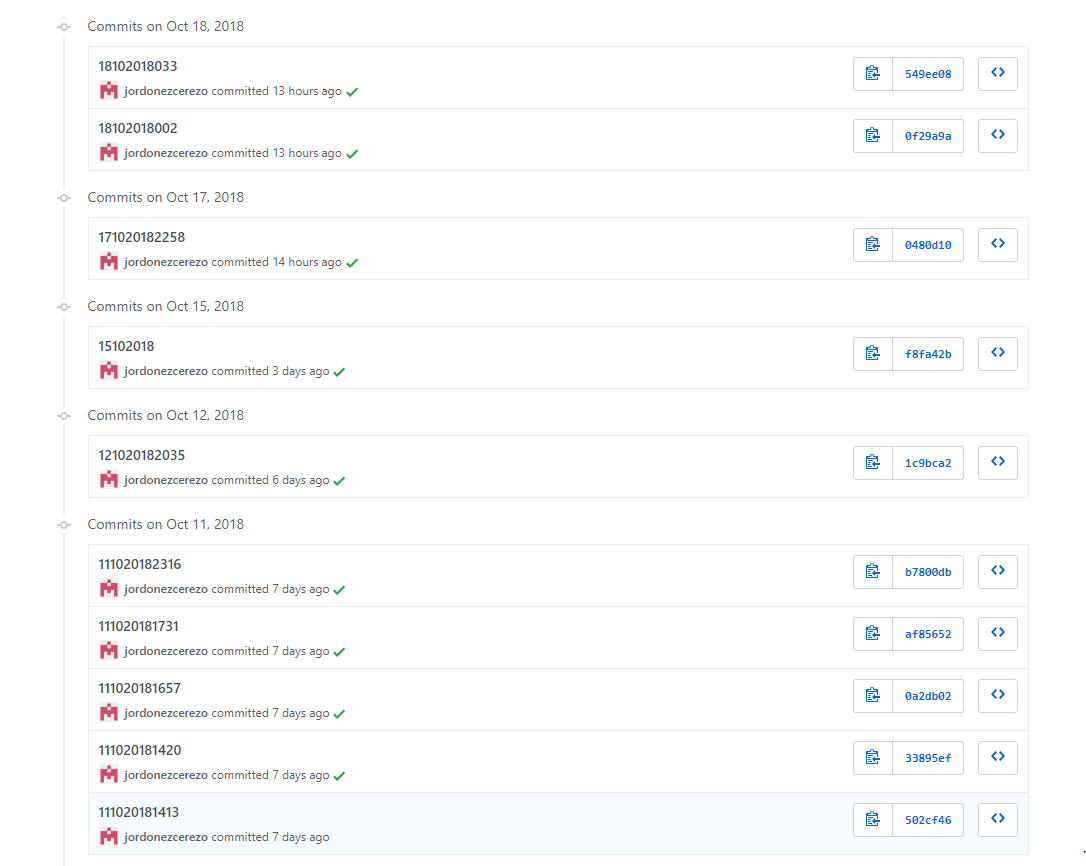
\includegraphics[trim = 0mm 0mm 0mm 0mm, clip,scale=0.5]{imagenes/Introduction/CapturaGit}
	\caption{Commits GitHub.}
	\label{fig:capturaGit}
\end{figure}

Para el buen cumplimiento de los objetivos planteados en primera instancia, y teniendo en cuenta la diferente localización de los componentes del trabajo, se hizo necesario el planteamiento de reuniones semanales (normalmente los Viernes) donde se pusiese en común lo trabajado durante la semana y se fijasen los siguientes objetivos. \newline

Para ello, se utilizo la herramienta se software libre llamada "Appear.in", la cuál ofrece videoconferencias entre varios usuarios al mismo instante (figura \ref{fig:appear}). 

\begin{figure}[H]
	\center
	
\includegraphics[trim = 0mm 0mm 0mm 0mm, clip,scale=0.3]{imagenes/Introduction/appear}
	\caption{Appear.in.}
	\label{fig:appear}
\end{figure}

\subsection{Estructura de la memoria}

La memoria está dividida en tres capítulos o partes diferenciadas. \newline
En la sección \ref{sec:Estado_arte} se explicará brevemente toda la parte teorica y conocimientos necesarios para el entendimiento del presente trabajo. Además se comentará la evolución hasta la actualidad de algunos sistemas propuestos.\newline

En la sección \ref{sec: BalancingRobot} se abordará en problema del Balancing Robot, y se diferenciara entre una parte de diseño y una parte de implementación, haciendo especial hincapié en el control PID que será utilizado en el capítulo siguiente. El Balancing Robot será capaz de mantenerse estable sobre dos ruedas horizontales.\newline

En la sección \ref{sec: Cuadricoptero} se abordará el problema de visión a bordo de un cuadricóptero. 
Una vez conseguidos los objetivos necesarios en la sección anterior, un cuadricoptero será capaz de seguir una pelota roja, por lo que se implementará el protocolo necesario para ello. \newline

Para terminar, en la sección \ref{sec: Conclusiones} se expondrán las conclusiones derivadas del trabajo completo, así como un posible trabajo futuro, errores a corregir, etc.   
%
%\input{capitulos/02_EspecificacionRequisitos}
%
%\input{capitulos/03_Planificacion}
%
%\input{capitulos/04_Analisis}
%
%\input{capitulos/05_Diseno}
%
%\input{capitulos/06_Implementacion}
%
%\input{capitulos/07_Pruebas}
%
%\input{capitulos/08_Conclusiones}
%
%%\chapter{Conclusiones y Trabajos Futuros}
%
%
%%\nocite{*}
%\bibliography{bibliografia/bibliografia}\addcontentsline{toc}{chapter}{Bibliografía}
%\bibliographystyle{miunsrturl}
%
%\appendix
%\input{apendices/manual_usuario/manual_usuario}
%%\input{apendices/paper/paper}
%\input{glosario/entradas_glosario}
% \addcontentsline{toc}{chapter}{Glosario}
% \printglossary
\chapter*{}
\thispagestyle{empty}

\end{document}
